% This is samplepaper.tex, a sample chapter demonstrating the
% LLNCS macro package for Springer Computer Science proceedings;
% Version 2.20 of 2017/10/04
%
\documentclass[runningheads]{llncs}
%
\usepackage{graphicx}
\graphicspath{{images/}}
% Used for displaying a sample figure. If possible, figure files should
% be included in EPS format.
\usepackage{amsmath}
\usepackage[hyphens, spaces]{url}
% If you use the hyperref package, please uncomment the following line
% to display URLs in blue roman font according to Springer's eBook style:
\usepackage{hyperref}
\renewcommand\UrlFont{\color{blue}\rmfamily}
\usepackage[linesnumbered, ruled]{algorithm2e}
\usepackage{mathtools} % for coloneqq
\usepackage{subfig}
\usepackage{booktabs}

\newcommand{\round}[1]{\ensuremath{\lfloor#1\rceil}}
\DeclareMathOperator*{\argmin}{arg\,min}

\begin{document}
%
\title{An efficient new static scheduling heuristic for accelerated architectures\thanks{Supported by the Engineering and Physical Sciences Research Council.}}
%
%\titlerunning{Abbreviated paper title}
% If the paper title is too long for the running head, you can set
% an abbreviated paper title here
%
\author{Thomas McSweeney\inst{1}\orcidID{0000-0001-9866-2229} }
%
\authorrunning{T. McSweeney}
% First names are abbreviated in the running head.
% If there are more than two authors, 'et al.' is used.
%
\institute{University of Manchester, Manchester, UK, M13 9PL \\
	\email{thomas.mcsweeney@postgrad.manchester.ac.uk} }
%
\maketitle              % typeset the header of the contribution
%
\begin{abstract}

Heterogeneous architectures which make use of {\em Graphics Processing Units} (GPUs) for general computations, in addition to multicore CPUs, are increasingly common in high-performance computing. However many of the existing methods for scheduling precedence-constrained tasks on such platforms were intended for more diversely heterogeneous clusters, such as the classic {\em Heterogeneous Earliest Finish Time} (HEFT) heuristic. We propose a new static scheduling heuristic called {\em Heterogeneous Optimistic Finish Time} (HOFT) which has the same structure as HEFT but exploits the low degree of heterogeneity of CPU-GPU platforms. Through extensive experimentation using custom software for simulating task scheduling problems on user-defined CPU-GPU platforms, we show that HOFT can obtain schedules at least $5\%$ shorter than HEFT's for medium to large-sized numerical linear algebra application task graphs and around $2\%$ shorter on average for a large collection of randomly-generated graphs.   


\keywords{GPU computing  \and static scheduling \and task-based programming.}
\end{abstract}


\section{Introduction}
\label{sect.intro}

Modern {\em High-Performance Computing} (HPC) machines typically comprise hundreds or even thousands of networked nodes. These nodes are increasingly likely to be {\em heterogeneous}, hosting one or more GPUs in addition to multicore CPUs. For example, Summit, which currently heads the Top500\footnote{\href{https://www.top500.org/}{{\tt \small https://www.top500.org/}}} list of the world's fastest supercomputers, comprises over $4000$ nodes, each with two 22-core IBM Power9 CPUs and six NVIDIA Tesla V100 GPUs. 

Task-based parallel programming is a paradigm that aims to harness this processor heterogeneity. Here a program is described as a collection of {\em tasks}---logically discrete atomic units of work---with {\em precedence constraints} that define the order in which they can be executed. This can be expressed in the form of a graph, where each vertex represents a task and edges the precedence constraints between them. We are interested only in the case when such task graphs are {\em Directed Acyclic Graphs} (DAGs)---directed and without any cycles.  

The immediate question is, how do we find the optimal way to assign the tasks to a set of heterogeneous resources while still respecting the precedence constraints? In other words, what {\em schedule} should we follow? This DAG scheduling problem is known to be NP-complete, even for homogeneous processors \cite{topcuoglu2002performance}, so typically we must rely on heuristic solutions that give us reasonable solutions in a reasonable time.

A fundamental distinction is made between {\em static} and {\em dynamic} scheduling problems. Static schedules are fixed before execution based on the information available at that time, whereas dynamic schedules are determined during runtime. There are generic advantages and disadvantages to both: static scheduling makes greater use of the data so is superior when it is sufficiently accurate, whereas dynamic scheduling uses more recent data. In practice task scheduling is usually handled by a {\em runtime system}, such as OmpSs \cite{duran2011ompss}, PaRSEC \cite{bosilca2013parsec}, or StarPU \cite{augonnet2011starpu}. Most such systems analyze data gathered during previous executions to predict task execution and data transfer times at runtime. On a single machine this is tricky since shared buses make estimating available bandwidth difficult and the possibility of asynchronous data transfers complicates matters further. Hence at present dynamic scheduling is typically preferred and many runtime systems do not permit static scheduling at all. However static schedules can be surprisingly robust, even when the estimates used are poor \cite{agullo2016}. Furthermore, superior performance can be achieved in dynamic environments by modifying an existing static schedule, rather than computing a new one from scratch \cite{ZHENG20131673}. 

In this paper we therefore focus on the problem of finding good static schedules for multicore and GPU platforms. To facilitate this investigation, we developed an open-source software simulator which allows users to simulate the static scheduling of arbitrary task DAGs on arbitrary CPU-GPU platforms, without worrying about the time or energy usage constraints imposed by real systems. Using this, we evaluate and optimize HEFT for these environments.  
% maybe add something like "with the understanding that these can be used as a basis for better dynamic schedules..."
% really want to emphasize the point here that the aim is to cheaply find a good static schedule so can use that as a jumping off point.

HEFT comprises two phases: a {\em task prioritization} phase in which the order tasks are to be scheduled is determined and a {\em processor selection} phase in which they are actually assigned to the processing resources. In this article we introduce HOFT, which follows the HEFT framework but modifies both phases, without significantly increasing the complexity of the algorithm. HOFT works by first computing a table of {\em optimistic} estimates of the earliest possible times all tasks can be completed on both processor types and using this to guide both phases. Simulations with real and randomly-generated DAGs on both single and multiple GPU target platforms suggest that HOFT is always at least competitive with HEFT and on average obtains schedule makespans around $3\%$ smaller.          

Explicitly, the two main contributions of this paper are:
\begin{enumerate}	
	\item A new static scheduling heuristic that is optimized specifically for accelerated heterogeneous architectures;
	\item Open-source simulation software that allows researchers to implement and evaluate their own scheduling methods for user-defined CPU-GPU platforms in a fast and reproducible manner.
\end{enumerate} 
The remainder of this paper is structured as follows. In Section \ref{sect.lit_review} we summarize the relevant existing literature, before explicitly defining the simulation model we use to study the static task scheduling problem and software we have created which implements this in Section \ref{sect.simulator}. We then describe HEFT in detail in Section \ref{sect.HEFT}, including also benchmarking results with our simulation model and a minor modification to the algorithm that we have found to perform well. In Section \ref{sect.hoft} we describe our new HOFT heuristic, before detailing the numerical experiments that we undertook to evaluate its performance in Section \ref{sect.results}. Finally in Section \ref{sect.conclusion} we state our conclusions from this investigation and outline future work that we believe may be useful.
 
% TODO: need to trim as much fat from here as possible.
\section{Related work}
\label{sect.lit_review}

Broadly, static scheduling methods can be divided into three categories: mathematical programming, guided-random and heuristics. (Note this taxonomy is our own.) The first is based on formulating the scheduling problem as a mathematical program and solving it using any applicable solver. See, for example, Kumar's constraint programming formulation in \cite{kumar:tel-01538516}. However these are usually so computationally expensive that they are restricted to very small DAGs. Guided-random is a term used for any method that generates a large population of potential schedules and then selects the best among them. Typically these are more general optimization schemes such as genetic algorithms which are refined for the task scheduling problem. As a rule, these methods tend to find very high-quality schedules but take a long time to do so; for example, a comparison by Braun et al. found that genetic algorithms usually obtained superior schedules to all other alternatives considered but were up to 300 times as expensive \cite{BRAUN2001810}. 

Heuristics are the most popular approach in practice as they are often both competitive with the alternatives and considerably faster. In turn {\em listing} heuristics are the most popular kind. They follow a two-phase structure: an ordered list of all tasks is first constructed (task prioritization) and they are then scheduled in this order according to some rule (processor selection). HEFT is the most prominent example: all tasks are prioritized according to their {\em upward rank} and then scheduled on the processor expected to complete their execution at the earliest time; a fuller description is given in Section \ref{sect.HEFT}. Canon et al. \cite{canon2008comparative} compared twenty different task scheduling heuristics and found that HEFT was almost always among the best in terms of both schedule makespan and robustness.

%There are in turn three occasionally overlapping types. {\em Clustering} heuristics work by first grouping all tasks in the DAG and then scheduling each cluster to a single processing resource, with the goal of reducing communication costs \cite{topcuoglu2002performance}. The drawback tends to be that the clustering step is expensive. {\em Duplication-based} heuristics also attempt to reduce communication costs, by ensuring that communicating tasks are scheduled on the same resource even if this requires them to be duplicated---i.e., the same task may be redundantly scheduled in more than one place \cite{duplication}. They can often be superior to alternatives in terms of schedule quality \cite{hcpfd} but they generally also have very high time-complexity bounds \cite{topcuoglu2002performance} since controlling the amount of duplication is tricky: too much can lead to the system becoming clogged, with duplicated tasks obstructing the optimal scheduling of others. 

Many modifications of HEFT have been proposed in the literature, such as HEFT {\em with lookahead} from Bittencourt, Sakellariou and Madeira \cite{bittencourt10}, which has the same task prioritization phase but schedules all tasks on the resources estimated to minimize the completion time of their {\em children}. This has the effect of increasing the time complexity of the algorithm so, in an attempt to incorporate a degree of lookahead into the HEFT framework without increasing the cost, Arabnejad and Barbosa proposed {\em Predict Earliest Finish Time} (PEFT) \cite{arabnejad14}. The main innovation is that rather than just minimizing the completion time of a task during processor selection, we instead minimize an {\em optimistic} estimate of the time it will take to execute the entire DAG once the task has been scheduled.

The majority of methods for static DAG scheduling in heterogeneous computing were originally intended for grid or cluster platforms but are also applicable to multicore and GPU, albeit perhaps with different behavior. Agullo et al. \cite{agullo2016} consider how well-suited static scheduling is for CPU-GPU environments in particular. After extensive experimentation on real systems they concluded that static schedules can be stable even when the estimates used to compute them are inaccurate. Furthermore, they found that incorporating static features into dynamic schedules often improves their performance. 

The most similar previous work to this is by Shetti, Fahmy and Bretschneider \cite{shetti2013optimization}, in which they propose the HEFT-NC ({\em No Cross}) heuristic as an optimization of HEFT for CPU-GPU environments. Although this is also our aim, the new HOFT heuristic differs significantly from HEFT-NC in both the task prioritization and processor selection phases of the algorithm. 

%(However, it can be viewed conceptually as an extension of HEFT-NC that implicitly incorporates communication costs when computing task rankings and uses a different mechanism in order to reduce what the original authors call {\em crossover}; see Section \ref{sect.hoft} for a full description of HOFT.)   


\section{Simulation model}
\label{sect.simulator}

In this paper we use a simulation model to study the static task scheduling problem for multicore and GPU environments. This is implemented in {\tt Python} and simulates the scheduling of user-defined DAGs on user-defined CPU-GPU platforms. The source code is available at the following Github repository: 
\begin{center}
	\href{https://github.com/mcsweeney90/heterogeneous_optimistic_finish_time}{{\tt \small https://github.com/mcsweeney90/heterogeneous\_optimistic\_finish\_time}}.
\end{center} 
The code used to generate all results presented in this paper is available in the folder {\tt simulator/scripts} so interested researchers may repeat our experiments for themselves. In addition, users may make modifications to the simulator that they believe will more accurately reflect their own target environment. 

To build the simulation model we gathered data from a single heterogeneous node of a local computing cluster. This comprises four octacore Intel (Skylake) Xeon Gold 6130 CPUs running at 2.10GHz with 192GB RAM and four Nvidia V100-SXM2-16GB (Volta) GPUs, each with 16GB GPU global memory, 5120 CUDA Cores and NVLink interconnect. We used {\em Basic Linear Algebra Subroutine} (BLAS) \cite{Dongarra:1990:SLB:77626.79170} kernels for these data-gathering experiments because they are widely-used in scientific computing applications.

\subsection{Mathematical model}
\label{subsect.mathematical_model}

The simulator software implements the following mathematical model of the problem. Suppose we have a task DAG $G$ consisting of $n$ tasks and $e$ edges that we wish to execute on a target platform $H$ comprising $P$ processing resources of two types, $P_C$ CPU resources and $P - P_C = P_G$ GPU resources. In keeping with much of the related literature and based on current programming practices, we consider CPU cores individually but regard entire GPUs as discrete \cite{agullo2016}. For example, a node comprising 4 GPUs and 4 octacore CPUs would be viewed as 4 GPU resources and $4 \times 8 = 32$ CPU resources.   

We assume that all tasks $t_1, \dots, t_n$ are atomic and cannot be divided across multiple resources or aggregated to form larger tasks. Further, all resources can only execute a single task at any one time and can in principle execute all tasks, albeit with different processing times. In our experiments, we found that the spread of BLAS kernel processing times on CPU cores and GPUs was usually tight, with the standard deviation often being two orders of magnitude smaller than the mean. Thus we assume that all task execution times on all processing resources of a single type are identical. In particular, this means that each task has only two possible {\em computation costs}: a CPU execution time $w_C(t_i)$ and a GPU execution time $w_G(t_i)$. When necessary, we denote by $w_{im}$ the processing time of task $t_i$ on the specific resource $p_m$.

The {\em communication cost} between task $t_i$ and its child $t_j$ is the length of time between when execution of $t_i$ is complete and execution of $t_j$ can begin, including all relevant latency and data transfer times. Since this depends on which processing resource executes each task, we view this as a function $c_{ij}(p_m, p_n)$. Based on our analysis of the time taken from when a specific processing resource completed execution of a task and another was able to begin execution of a child task on our data-gathering node, we assume in our simulation model that there are only four possible communication costs between tasks $t_i$ and $t_j$: $c_{ij}(C, C)$, from a CPU to a different CPU; $c_{ij}(C, G)$, from CPU to GPU; $c_{ij}(P, C)$, from GPU to CPU; and $c_{ij}(G, G)$ from GPU to a different GPU. 
%Of course, this assumption is not representative of all possible CPU-GPU memory architectures but is intended to be reasonable for a typical heterogeneous HPC node today. 

A {\em schedule} is a mapping from tasks to processing resources, as well as the precise time at which their execution should begin. Our goal is to find a schedule which minimizes the {\em makespan} of the task graph, the total execution time of the application it represents. Although we assume that all computation and communication costs represent time, they could be any other cost we wish to minimize, such as energy consumption, so long as this is done consistently. We do not however consider the simultaneous optimization of two or more different types of costs. A task with no successors is called an {\em exit} task. Once all tasks have been scheduled, the makespan is easily computed as the earliest time all exit tasks have been executed.

\subsection{Testing environments}
\label{subsect.testing_environment}

In the numerical experiments described later in this article, we consider two simulated target platforms: {\em Single GPU}, comprising 1 GPU and 1 octacore CPU, and {\em Multiple GPU}, comprising 4 GPUs and 4 octacore CPUs. The latter represents the node we used to guide the development of our simulator and the former is considered in order to study how the number of GPUs affects performance. We follow the convention that a CPU core is dedicated to managing each of the GPUs \cite{augonnet2011starpu}, so these two platforms are actually assumed to comprise 7 CPU and 1 GPU resources, and 28 CPU and 4 GPU resources, respectively. Based on our exploratory experiments, we make two further assumptions. First, since communication costs between CPU resources were negligible relative to all other combinations, we assume they are zero---i.e., $c_{ij}(C, C) = 0, \forall i, j$. Second, because CPU-GPU communication costs were very similar to the corresponding GPU-CPU and GPU-GPU costs, we take them to be identical---i.e., $c_{ij}(C, G) = c_{ij}(G, C) = c_{ij}(G, G), \forall i, j$. Again, these assumptions will not be representative of all architectures, but the simulator software allows users who wish to repeat our experiments to do so for more accurate representations of their own target platforms. 

We consider the scheduling of two different sets of DAGs. The first consists of ten DAGs comprising between $35$ and $22,100$ tasks which correspond to the {\em Cholesky factorization} of $N \times N$ tiled matrices, where $N = 5, 10, 15, \dots, 50$. In particular, the DAGs are based on a common implementation of Cholesky factorization which uses {\tt GEMM} (matrix multiplication), {\tt POTRF} (Cholesky factorization), {\tt SYRK} (symmetric rank-$k$ update) and {\tt TRSM} (triangular solve) BLAS kernels \cite{Dongarra:1990:SLB:77626.79170}. All task CPU/GPU processing times are means of 1000 real timings of that task kernel. Likewise, communication costs are sample means of real communication timings between the relevant task and resource types. All numerical experiments were performed for tile sizes $128$ and $1024$; which was used will always be specified where results are presented. Those sizes were chosen as they roughly mark the upper and lower limits of tile sizes typically used for CPU-GPU platforms.

The standard way to quantify the relative amount of communication and computation represented by a task graph is the {\em computation-to-communication ratio} (CCR), the mean computation cost of the DAG divided by the mean communication cost. For the Cholesky DAGs, the CCR was about 1 for tile size 128 and about 18 for tile size 1024, with minor variation depending on the total number of tasks in the DAG. 
% CCR $\coloneqq n \sum_{i, j}\overline{c_{ij}}  / e\sum_{i} \overline{w_i}$ - haven't defined mean computation and communication costs yet...

We constructed a set of randomly-generated DAGs with a wide range of CCRs, based on the topologies of the 180 DAGs with 1002 tasks from the {\em Standard Task Graph} (STG) set \cite{Tobita2002}. Following the approach in \cite{canon2018}, we selected GPU execution times for all tasks uniformly at random from $[1, 100]$ and computed the corresponding CPU times by multiplying by a random variable from a Gamma distribution. To consider a wide range of potential applications, we made two copies with different parameters for the distribution: one with mean and standard deviation 5 and another with both taken to be $50$ instead. These values roughly correspond to what we observed in our benchmarking of BLAS kernels with tile sizes $128$ and $1024$, respectively. Finally, for both parameter regimes, we made three copies of each DAG and for each copy randomly generated communication costs such that the CCR fell into one of the intervals $[0, 10]$, $[10, 20]$ and $[20, 50]$. Thus in total the random DAG set contains $1080$ DAGs.  
% The idea is that this will also cover other architectures implicitly...
% "We chose a larger value for the scale in order to also implcitly consider other architectures..."
% Change the range to make it a parameter?



\section{HEFT}
\label{sect.HEFT}

Recall that as a listing scheduler HEFT comprises two phases, an initial {\em task prioritization} phase in which the order all tasks are to be scheduled is determined and a {\em processor selection} phase in which the processing resource each task is to be scheduled on is decided. Here we describe both in order to give a complete description of the HEFT algorithm. Then in Section \ref{subsect.benchmarking} we benchmark HEFT's performance using our simulation model. Finally, in Section \ref{subsect.heft_WM} we describe a simple modification to the HEFT algorithm that we found to be effective.      

The {\em critical path} of a DAG is the longest path through it, and is important because it gives a lower bound on the optimal schedule makespan for that DAG. Heuristics for homogeneous platforms often use the {\em upward rank}, the length of the critical path from that task to an exit task, including the task itself \cite{topcuoglu2002performance}, to determine priorities. Computing the critical path is not straightforward for heterogeneous platforms so HEFT extends the idea by using {\em mean} values instead. Intuitively, the task prioritization phase of HEFT can be viewed as an approximate dynamic program applied to a simplified version of the task DAG that uses mean values to set all weights.

More formally, we first define the {\em mean execution cost} of all tasks $t_i$ through
\begin{equation}
\label{eq.avg_comp}
\overline{w_i} \coloneqq \sum_{m = 1}^{P} \frac{w_{im}}{P} = \frac{w_C(t_i) P_C + w_G(t_i) P_G}{P},
\end{equation}  
where the second expression is how $\overline{w_i}$ would be computed under the assumptions of our model. Likewise, the {\em mean communication cost} $\overline{c_{ij}}$ between $t_i$ and $t_j$ is then the average of all such costs over all possible combinations of resources,
\begin{align}
\label{eq.avg_comm}
\overline{c_{ij}} = \frac{1}{P^2}\sum_{m, n} c_{ij}(p_m, p_n) = \frac{1}{P^2}\sum_{k, \ell \in \{ C, G \}} A_{k\ell} c_{ij}(k, \ell),
\end{align}
where $A_{CC} = P_C(P_C - 1)$, $A_{CG} = P_C P_G = A_{GC}$, and $A_{GG} = P_G(P_G - 1)$. 
For all tasks $t_i$ in the DAG, we define their upward ranks $rank_u(t_i)$ recursively, starting from the exit task(s), by
\begin{align}
\label{eq.upward_rank}
rank_u(t_i) = \overline{w_i} + \max_{t_j \in Ch(t_i)} (\overline{c_{ij}} + rank_u(t_j)),
\end{align}
where $Ch(t_i)$ is the set of $t_i$'s immediate successors in the DAG. The task prioritization phase then concludes by listing all tasks in decreasing order of upward rank, with ties broken arbitrarily. 

The processor selection phase of HEFT is now straightforward: we move down the list and assign each task to the resource expected to complete its execution at the earliest time. Let $R_{m_i}$ be the earliest time at which the processing resource $p_m$ is actually free to execute task $t_i$, $Pa(t_i)$ be the set of $t_i$'s immediate predecessors in the DAG, and $AFT(t_k)$ be the time when execution of a task $t_k$ is actually completed (which in the static case is known precisely once it has been scheduled). Then the {\em earliest start time} of task $t_i$ on processing resource $p_m$ is computed through
\begin{align}
\label{eq.EST}
EST(t_i, p_m) = \max \bigg\{ R_{m_i}, \max_{t_k \in Pa(t_i)} (AFT(t_k) + c_{ki}(p_k, p_m)) \bigg\}
\end{align}
and the {\em earliest finish time} $EFT(t_i, p_m)$ of task $t_i$ on $p_m$ is given by 
\begin{align}
\label{eq.EFT}
EFT(t_i, p_m) = w_{im} + EST(t_i, p_m).
\end{align}
HEFT follows an {\em insertion-based} policy that allows tasks to be inserted between two that are already scheduled, assuming precedence constraints are still respected, so $R_{m_i}$ may not simply be the latest finish time of all tasks on $p_m$. A complete description of HEFT is given in Algorithm \ref{alg.HEFT}. HEFT has a time complexity of $O(P \cdot e)$. For dense DAGs, the number of edges is proportional to $n^2$, where $n$ is the number of tasks, so the complexity is effectively $O(n^2P)$ \cite{topcuoglu2002performance}. 
\begin{algorithm}	
	
	Set the computation cost of all tasks using \eqref{eq.avg_comp}
	
	Set the communication cost of all edges using \eqref{eq.avg_comm}
	
	Compute $rank_u$ for all tasks according to \eqref{eq.upward_rank}
	
	Sort the tasks into a priority list by non-increasing order of $rank_u$
	
	\For{task in list}
	{	
		
		\For{each resource $p_k$}
		{Compute $EFT(t_i, p_k)$ using \eqref{eq.EST} and \eqref{eq.EFT}}
		
		$p_m \coloneqq \argmin_k(EFT(t_i, p_k))$
		
		Schedule $t_i$ on the resource $p_m$ 
		
	}	
	\caption{HEFT.}
	\label{alg.HEFT}
\end{algorithm} 


\subsection{Benchmarking}
\label{subsect.benchmarking}

Using our simulation model, we investigated the quality of the schedules computed by HEFT for the Cholesky and randomly-generated DAG sets on both the single and multiple GPU target platforms described in Section \ref{sect.simulator}. The metric used for evaluation was the {\em speedup}, the ratio of the {\em minimal serial time} (MST)---the minimum execution time of the DAG on any single resource---to the makespan. Intuitively, speedup tells us how well the schedule exploits the parallelism of the target platform. Figure \ref{plot.heft_benchmark_cholesky} shows the speedup of HEFT for the Cholesky DAGs with tile size $128$. The most interesting takeaway is the difference between the two platforms. With multiple GPUs the speedup increases uniformly with the number of tasks until we see a small decline for the very largest DAG. But for a single GPU the speedup stagnates much more quickly. It is not clear to us why this is the case, but one possibility is that HEFT in some sense achieves the maximum amount of parallelism it is able to exploit on the single GPU platform for smaller DAGs than it does for the larger, more parallel multiple GPU platform. Results were broadly similar for Cholesky DAGs with tile size $1024$, with the exception that the speedup values were uniformly smaller, reaching a maximum of just over four for the multiple GPU platform. 
\begin{figure}
	\centering	
	\subfloat[Cholesky.]{\label{plot.heft_benchmark_cholesky}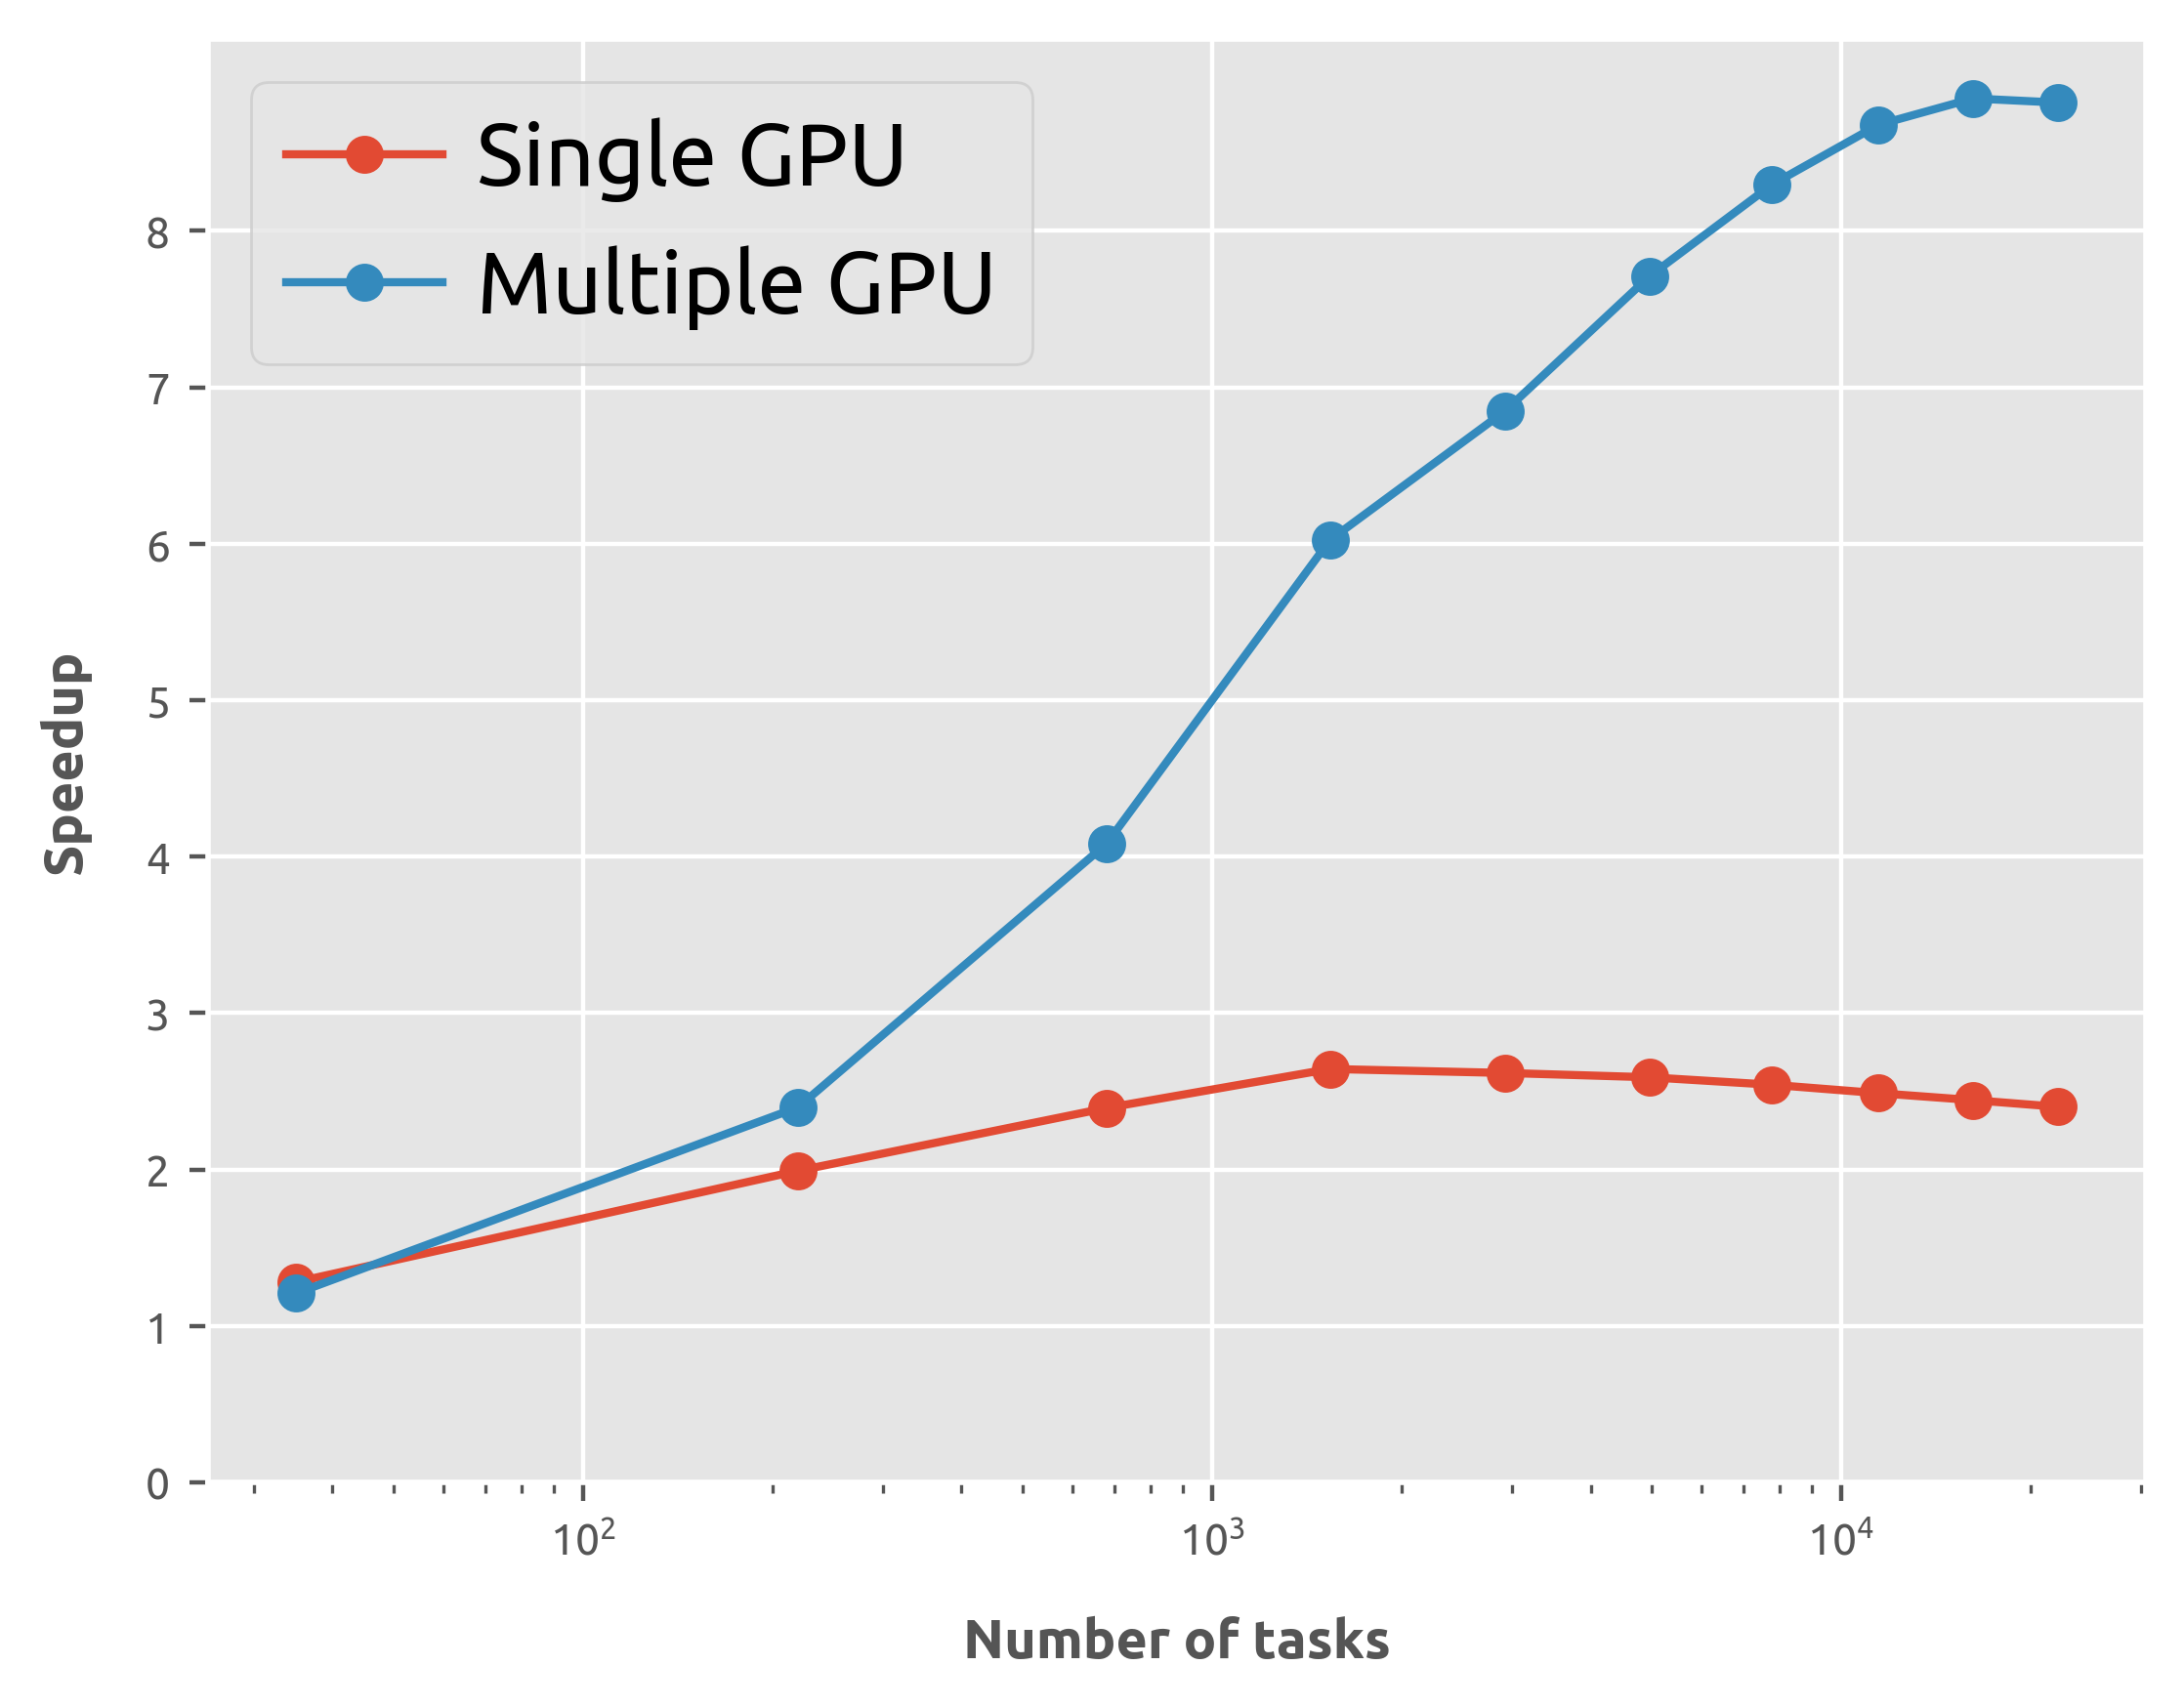
\includegraphics[scale=0.4]{cholesky_nb128_speedups.png}}
	\subfloat[Random.]{\label{plot.heft_benchmark_random}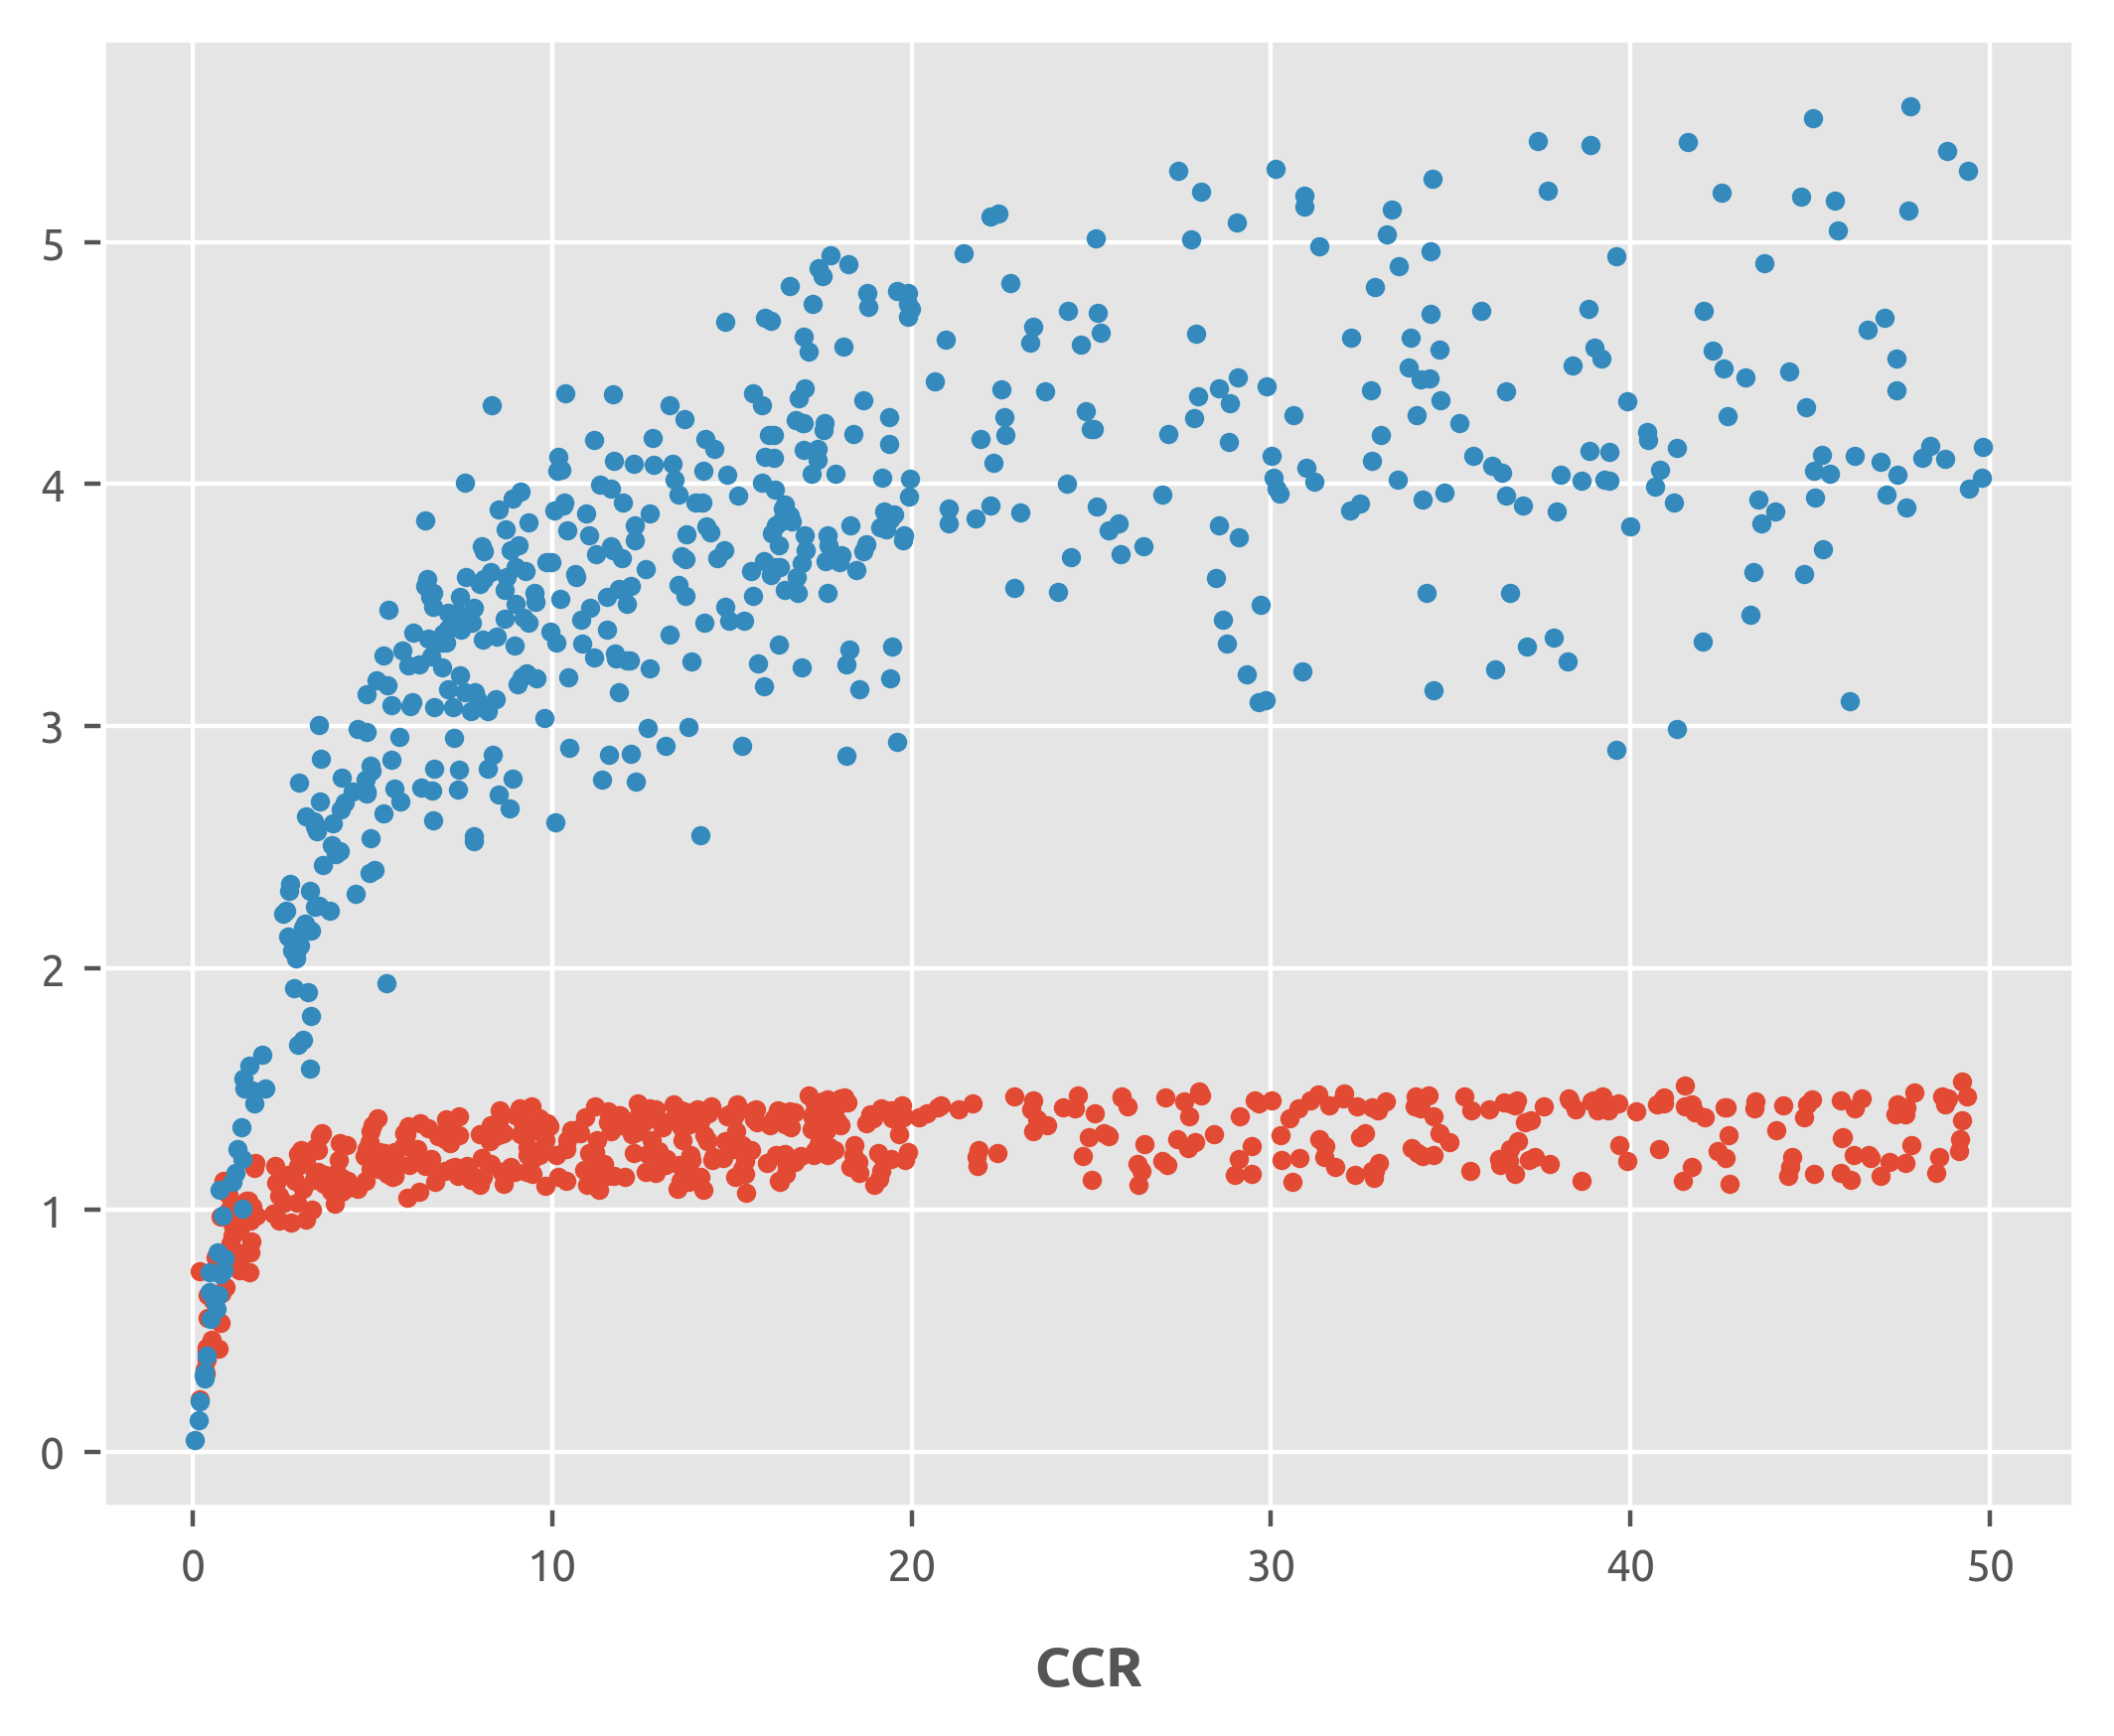
\includegraphics[scale=0.4]{random_speedups_high_acc.png}}
	\caption{Speedup of HEFT for Cholesky (tile size $128$) and random (high acceleration) DAG sets.}	
	\label{plot.heft_benchmark}
\end{figure}

Both similar and different behavior was apparent for the random DAG set. Figure \ref{plot.heft_benchmark_random} shows the speedups for all 540 {\em high acceleration} DAGs---for which CPU costs were generated using a Gamma distribution with mean and standard deviation 50---ordered by their CCRs. Results were broadly similar for the We see that the speedups for the single GPU platform are much smaller with a narrower spread compared to the other platform, as for the Cholesky DAGs. More surprising is that fact that HEFT sometimes returned a schedule with speedup less than one for DAGs with small CCR values, which we call a {\em failure} since this is obviously unwanted behavior. These failures were due to the greediness of the HEFT processor selection phase, which always schedules a task on the processing resource that minimizes its earliest finish time without considering the communication costs that may later be incurred by doing so. The effect is more pronounced when the CCR is low because the unforeseen communication costs are proportionally larger. A likely candidate for dealing with such cases would seem to be HEFT with lookahead \cite{bittencourt10}, but the additional computational cost of the modified algorithm proved impractical for our purposes. We investigated cheaper {\em sampling-based} selection phases that consider only a small selection of the child tasks---selected either at random or based on priorities---during the lookahead. These did reduce the failure probability slightly for DAGs with low CCR values but the improvement was only minor. An alternative to lookahead that may be useful is duplication-based heuristics \cite{duplication}.    



\subsection{HEFT-WM}
\label{subsect.heft_WM}

The implicit assumption underlying the use of mean values when computing task priorities in HEFT is that the probability of a task being scheduled on a processing resource is identical for all resources. But this is obviously not the case: if a task's GPU execution time is ten times smaller than its CPU execution time then it is considerably more likely to be scheduled on a GPU, even if not ten times so because of resource contention. This suggests that we should weight the mean values according to each task's {\em acceleration ratio} $r_i$, the CPU time divided by the GPU time. In particular, for each task $t_i$ we estimate its computation cost to be
\begin{equation}
\label{eq.avg_comp_wm}
\overline{w_i} = \frac{w_C(t_i) P_C + r_iw_G(t_i) P_G}{P_C + r_iP_G},
\end{equation}  
and for each edge (say, between tasks $t_i$ and $t_j$) the estimated communication cost is
\begin{equation}
\label{eq.avg_comm_wm}
\overline{c_{ij}} = \frac{A_{CC} \cdot c_{ij}(C, C) + A_{CG}\big(r_ic_{ij}(G, C) + r_jc_{ij}(C, G)\big) + r_ir_j A_{GG} \cdot c_{ij}(G, G) }{(r_iP_G + P_C) \cdot (r_jP_G + P_C)}. 
\end{equation}
We call the modified heuristic which follows Algorithm \ref{alg.HEFT} but uses \eqref{eq.avg_comp_wm} instead of \eqref{eq.avg_comp} and \eqref{eq.avg_comm_wm} instead of \eqref{eq.avg_comm} HEFT-WM (for {\em Weighted Mean}). We were unable to find any explicit references to this modification in the literature but given its simplicity we do not think it is a novel idea and suspect it has surely been used before in practice.  
% TODO: equation is hideous, tidy up the notation to make it more compact.
% TODO: end bit is stilted and reads oddly, change. Also, there might actually be a reference out there somewhere to weighting HEFT by the power of each processor so double check. 


\section{HOFT}
\label{sect.hoft}

If we disregard all resource contention, then we can easily compute the earliest possible time that all tasks can be completed assuming that they are scheduled on either a CPU or GPU resource, which we call the {\em Optimistic Finish Time} (OFT). More specifically, for $p, p' \in \{C, G\}$, we move forward through the DAG and build a table of OFT values by setting $OFT(t_i, p) = w_p(t_i)$, if $t_i$ is an entry task, and recursively computing     
\begin{align}
\label{eq.oft_table}
OFT(t_i, p) &= w_p(t_i) + \max_{t_j \in Pa(t_i)} \bigg \{ \min_{p'} \{ OFT(t_j, p') + \delta_{pp'} c_{ij} (p, p') \}  \bigg \}, 
\end{align}
for all other tasks, where $\delta_{pp'} = 1$ if $p = p'$ and $0$ otherwise. We use the OFT table as the basis for the task prioritization and processor selection phases of a new HEFT-like heuristic optimized for CPU-GPU platforms that we call {\em Heterogeneous Optimistic Finish Time} (HOFT). Note that computing the OFT table does not increase the order of HEFT's time complexity.  
% needs more detail here

Among several possible ways of using the OFT to compute a complete task prioritization, we found the most effective to be the following. First, define the weights of all tasks to be the ratio of the maximum and minimum OFT values,
\begin{align}
\label{eq.hoft_weights}
\overline{w_i} = \frac{\max\{ OFT(t_i, C), OFT(t_i, G) \}}{\min\{ OFT(t_i, C), OFT(t_i, G) \}}.
\end{align} 
Now assume that all edge weights are zero, $\overline{c_{ij}} \equiv 0, \forall i, j$, and compute the upward rank of all tasks with these values. Upward ranking is used to ensure that all precedence constraints are met. Intuitively, tasks with a strong preference for one resource type---as suggested by a high ratio---should be scheduled first. 

We also propose a new processor selection phase which proceeds as follows. Working down the priority list, each task $t_i$ is scheduled on the processing resource $p_{m}$ with the smallest EFT as in HEFT except when $p_m$ is not also the fastest resource type for that task. In such cases, let $p_f$ be the resource of the fastest type with the minimal EFT and compute 
\begin{align}
\label{eq.sm}
s_m \coloneqq EFT(t_i, p_f) - EFT(t_i, p_m),
\end{align}
the saving that we expect to make by scheduling $t_i$ on $p_m$ rather than $p_f$. Suppose that $p_m$ is of type $T_m \in \{C, G\}$. By assuming that each child task $t_j$ of $t_i$ is scheduled on the type of resource $T_j$ which minimizes its OFT, we define $E(Ch(t_i) | p_m)$ to be an optimistic estimate of the earliest finish time of all child tasks assuming that $t_i$ is scheduled on $p_m$. In particular, we compute
\begin{align}
\label{eq.oft_children}
E(Ch(t_i) | p_m) \coloneqq \max_{t_j \in Ch(t_i)} \Big( EFT(t_i, p_m) + c_{ij}(T_m, T_j) + w_{T_j}(t_j)\Big).
\end{align}
Likewise for $p_f$ we compute $E(Ch(t_i) | p_f)$. As in HEFT with lookahead, we call the estimates {\em optimistic} since they disregard the possible need to wait for other parent tasks to complete. Finally, if
\begin{align}
\label{eq.cross_condition}
s_m > E(Ch(t_i) | p_m) - E(Ch(t_i) | p_f)
\end{align}
we schedule task $t_i$ on $p_m$; otherwise, we schedule it on $p_f$. Intuitively, the processor selection always chooses the resource with the smallest EFT unless by doing so we expect to increase the earliest possible time at which all child tasks can be completed.

\begin{algorithm}	
	
	Compute the OFT table for all tasks using \eqref{eq.oft_table}
	
	Set the computation cost of all tasks using \eqref{eq.hoft_weights}
	
	Set the communication cost of all edges to be zero
	
	Compute $rank_u$ for all tasks according to \eqref{eq.upward_rank}
	
	Sort the tasks into a priority list by non-increasing order of $rank_u$
	
	\For{task in list}
	{	
		
		\For{each resource $p_k$}
		{Compute $EFT(t_i, p_k)$ using \eqref{eq.EST} and \eqref{eq.EFT}}	
		
		$p_m \coloneqq \argmin_k(EFT(t_i, p_k))$
		
		\If{$w_{im} \neq \min(w_C(t_i), w_G(t_i))$}{
			
		$p_f \coloneqq \argmin_k\big( EFT(t_i, p_k)| w_{ik} = \min(w_C(t_i), w_G(t_i)) \big)$	
		
		Compute $s_m$ using \eqref{eq.sm}.
		
		Compute $E(Ch(t_i) | p_m)$ and $E(Ch(t_i) | p_f)$ using \eqref{eq.oft_children}
		
		\If{\eqref{eq.cross_condition} holds}{Schedule $t_i$ on $p_m$}
		\Else{Schedule $t_i$ on $p_f$}			
		}
		
	}	
	\caption{HOFT.}
	\label{alg.HOFT}
\end{algorithm} 

\section{Simulation results}
\label{sect.results}

Figure \ref{plot.hoft_cholesky} shows the reduction in schedule makespan, as a percentage of the HEFT schedule, achieved by HOFT and HEFT-WM for the set of Cholesky DAGs, on both the single and multiple GPU target platforms. The overall trend for the multiple GPU platform is that HOFT improves relative to both HEFT variants as the number of tasks in the DAG grows larger; it is always better than standard HEFT for tile size 1024. For the single GPU platform, HOFT was almost always the best, except for the smallest DAGs and the largest DAG with tile size 128 (for which all three heuristics were almost identical). Interestingly, we found that the processor selection phase of HOFT never actually differed from HEFT's for these DAGs and so the task prioritization phase alone was key. 
\begin{figure}
	\centering	
	\subfloat[Tile size 128.]{\label{plot.hoft_cholesky_nb128}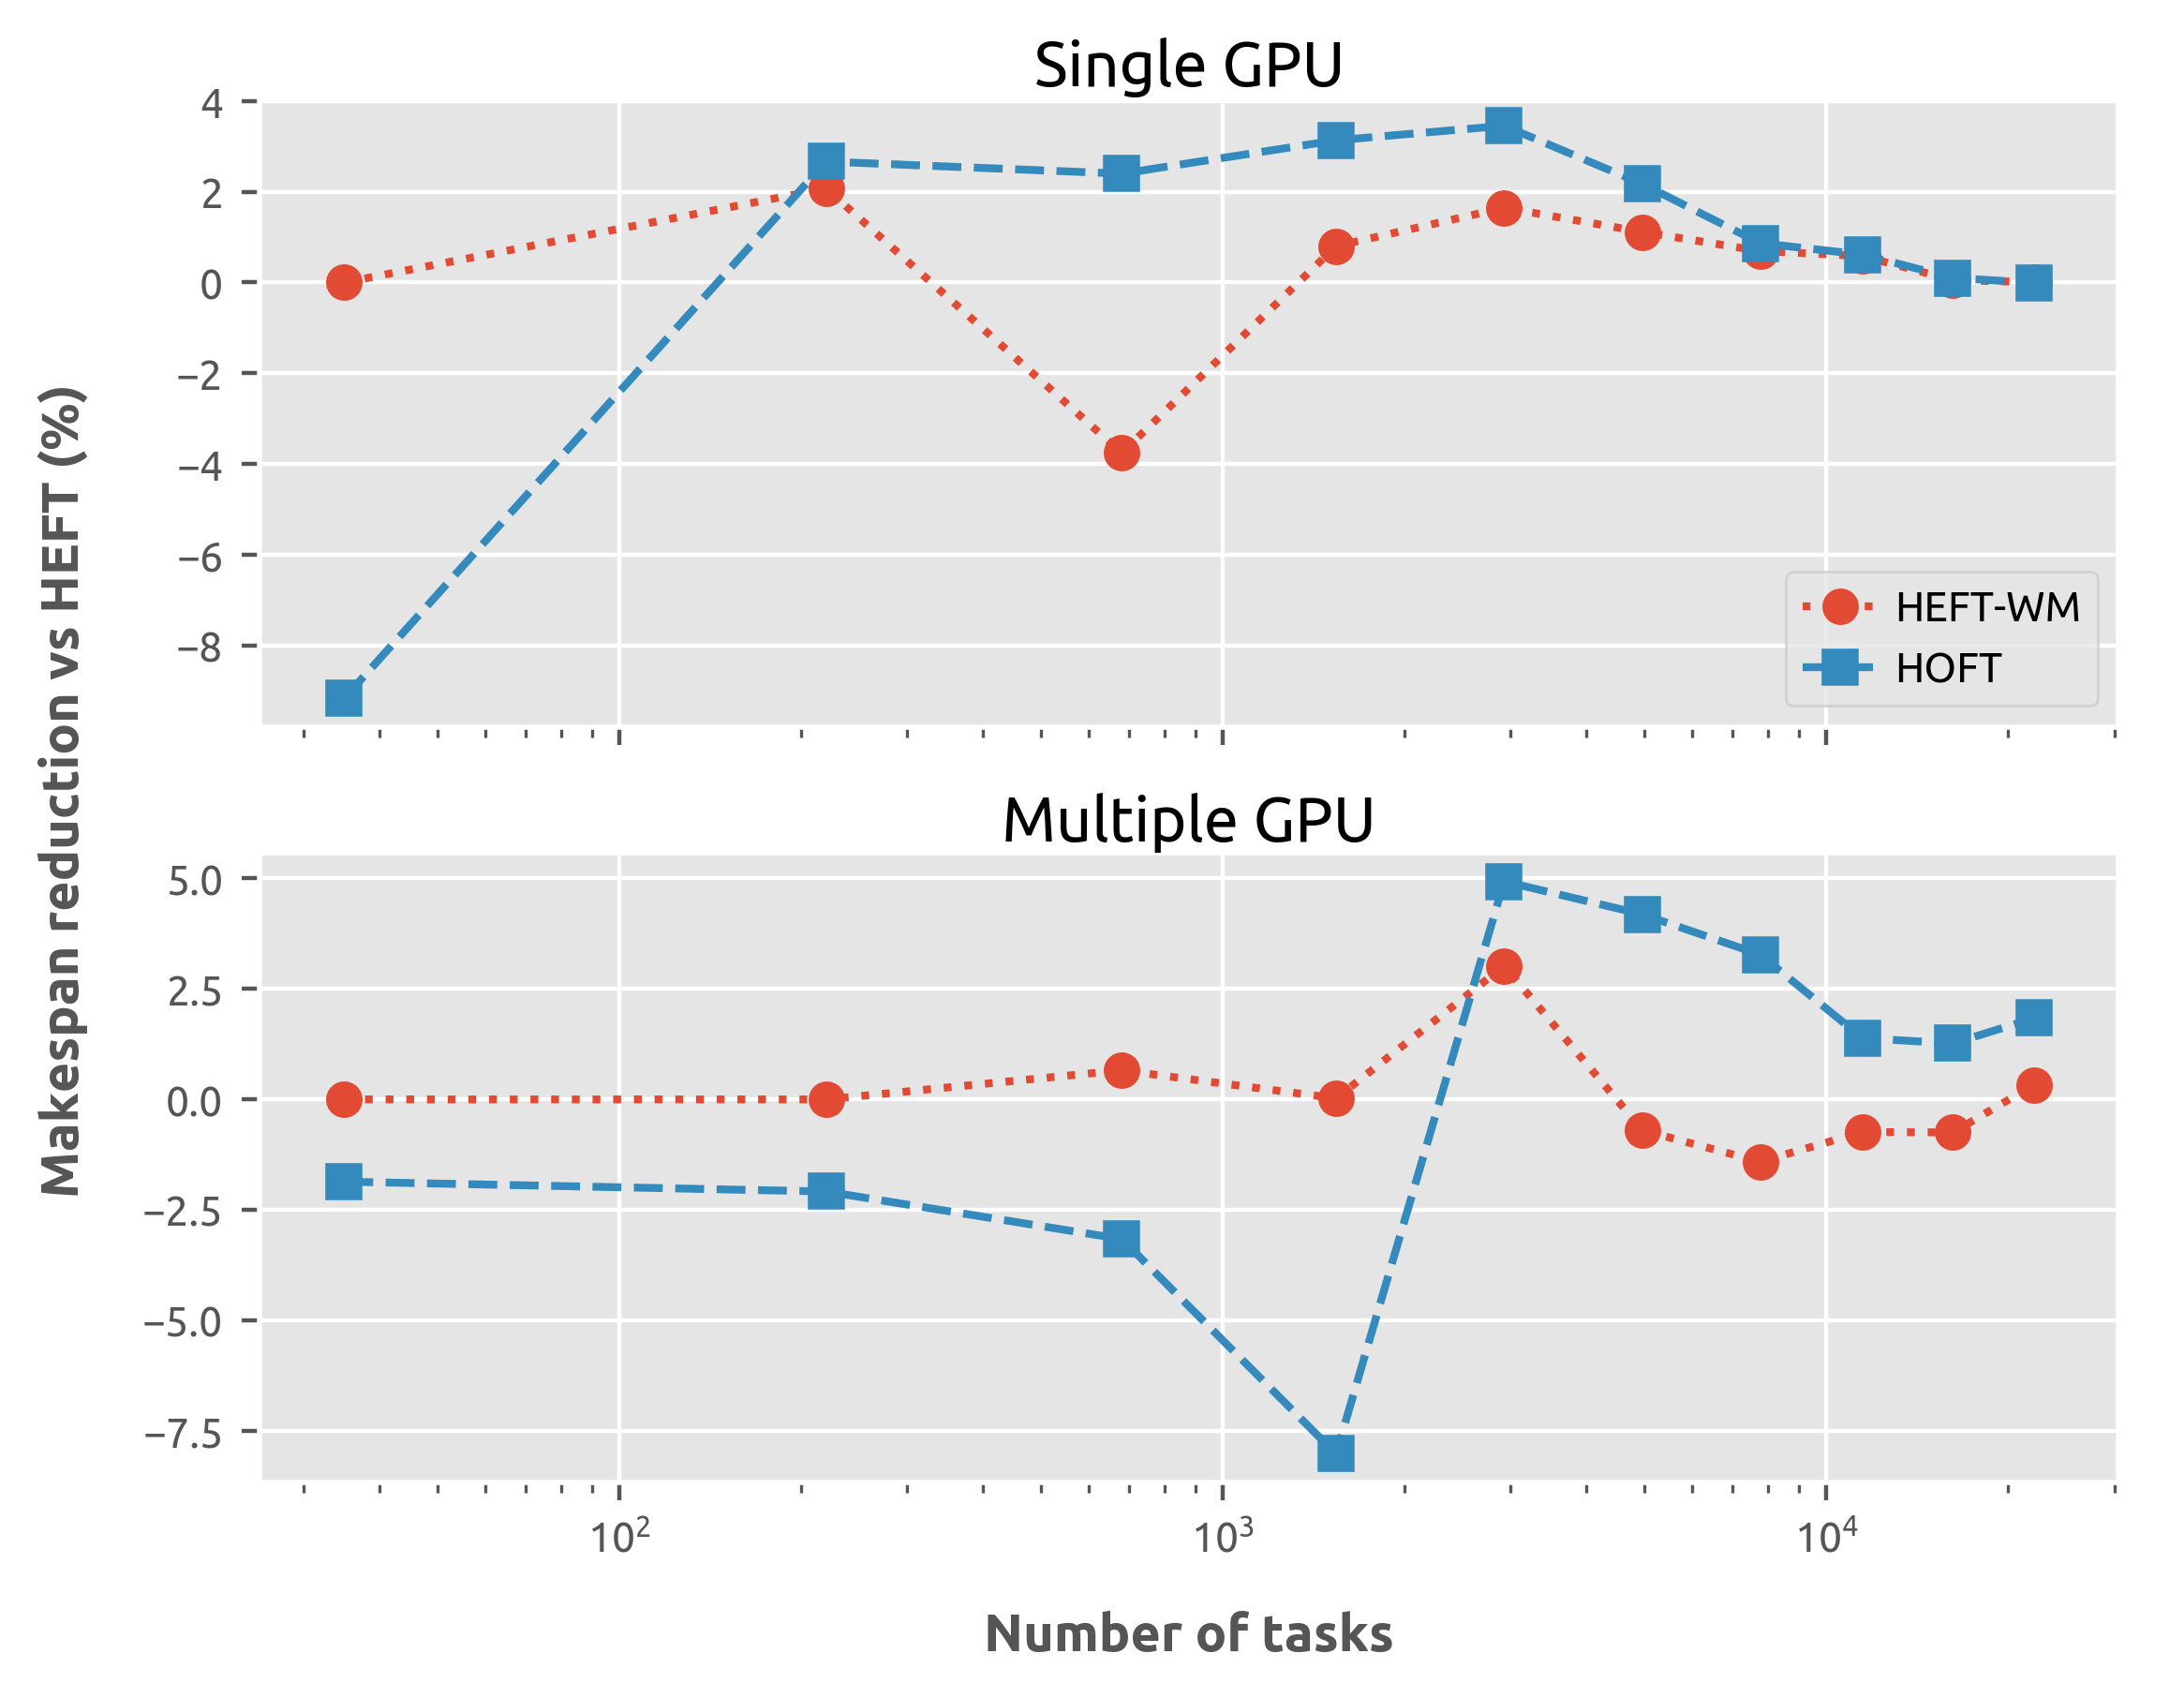
\includegraphics[scale=0.45]{hoft_speedup_cholesky_nb128.png}}
	\subfloat[Tile size 1024.]{\label{plot.hoft_cholesky_nb1024}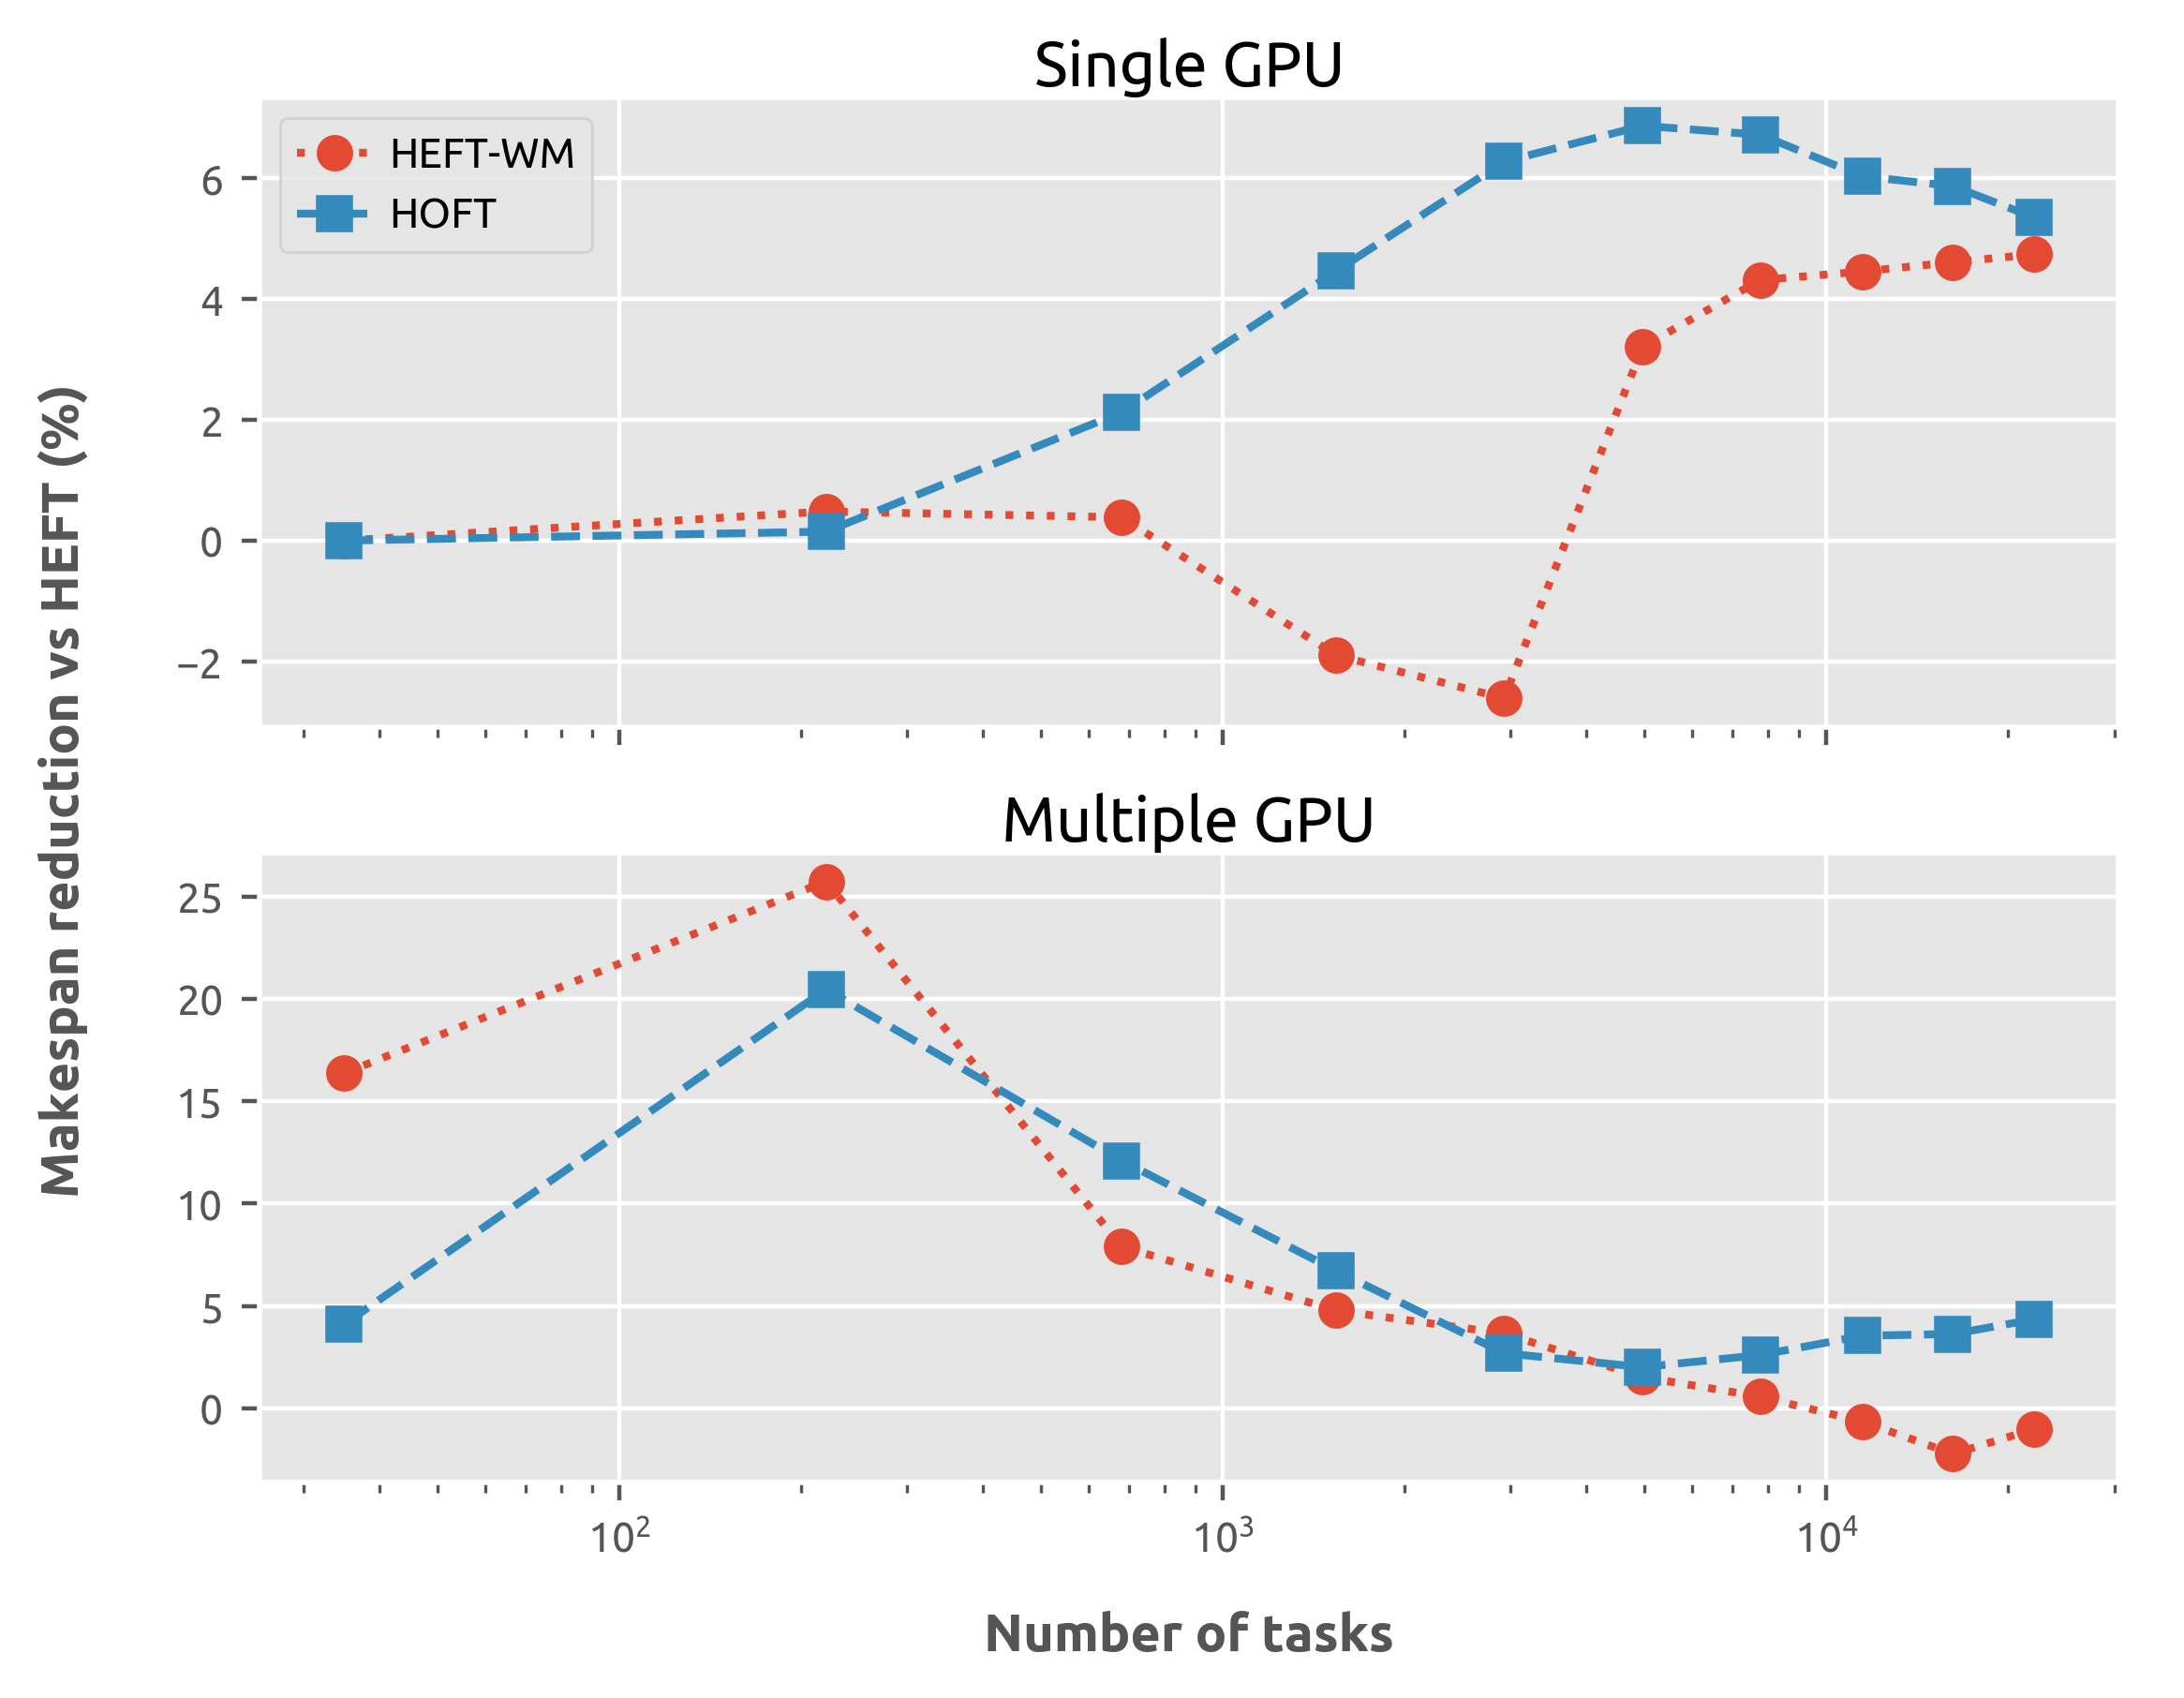
\includegraphics[scale=0.45]{hoft_speedup_cholesky_nb1024.png}}
	\caption{HEFT-WM and HOFT compared to HEFT for Cholesky DAGs.}	
	\label{plot.hoft_cholesky}
\end{figure} 

The relative performance of the heuristics was rather variable for the randomly-generated DAGs, depending on the target platform and acceleration regime. However both HOFT and HEFT-WM achieved smaller makespans than HEFT on average. Table X summarizes the results... Also included in the table is HOFT-WM, the heuristic obtained by using the HEFT-WM task prioritization phase with the HOFT processor selection.  
% TODO: tweak

  

%reduced the failure rate for DAGs with small CCRs, although never by more than $25\%$. Interestingly, none of the sets of DAGs for which the heuristics failed were ever entirely contained in another but there was normally a very high degree of overlap. Makespan variations when one failed but another did not were often very large. Disregarding all such cases to avoid distortion, the makespans of HOFT schedules were on average $2.3\%$ smaller than HEFT's on the multiple GPU platform, and $2.6\%$ smaller on the single GPU platform. Using either the HOFT task ranking or processor selection phase alone only resulted in average reductions about half as large. For HEFT-WM the average reductions across the random DAG set were $2.1\%$ and $1.5\%$ for the single and multiple GPU platforms respectively. By using the HOFT processor selection phase instead, we were able to increase both of those values to around about the same size as the HOFT average reductions, showing that it is useful no matter which task prioritization phase is used.


\section{Conclusions}
\label{sect.conclusion}

Taking the Cholesky and random DAG sets as a whole, HOFT improved on HEFT by an average of about $3\%$ on both the single and multiple GPU target platforms. For Cholesky DAGs in particular, makespan reductions for DAGs with more than $2000$ tasks were often even higher. In those cases, the reductions were entirely due to the alternative task prioritization phase, but for random DAGs the HOFT processor selection phase proved to be useful. Overall, the safest conclusion from our simulations is that HOFT appears to be at least competitive with---and often superior to---both standard HEFT and HEFT-WM for both single and multiple GPU target platforms. It should be noted that HEFT-WM also performed very well in our simulations and was almost invariably superior to the standard algorithm, suggesting that it should perhaps be the default in accelerated environments. 

As stated in Section \ref{sect.intro}, static schedules for multicore and GPU are most useful in practice as a foundation or guide for efficient dynamic schedules; this paper was concerned only with how such static schedules may be computed in the first place. Extending static scheduling to dynamic environments is often called {\em stochastic} scheduling, since the costs are usually modeled as random variables from some possibly unknown distribution. The goal is typically to find methods that bound variation in the schedule makespan, which is notoriously difficult given that Hagstrom \cite{hagstrom88} showed that even computing its probability distribution is a $\#P$-complete problem. Small-scale experimentation with existing stochastic scheduling heuristics, such as {\em Monte Carlo Scheduling} \cite{ZHENG20131673}, suggested to us that the main issue with adapting such methods for multicore and GPU is their cost, which can be much greater than computing the initial static schedule. Hence in future work we intend to investigate cheaper ways to make effective use of static schedules for real CPU-GPU platforms.  

%For example, for Cholesky factorization, exactly how the matrix is tiled---i.e., the size of the tiles and thus the tasks in the DAG---is usually guided by the architecture on which the algorithm is to be executed since GPUs are much better suited to large tile sizes than CPUs. In future work we intend to consider the related problem of how to construct more amenable task DAGs for a given application. More generally, we are assuming that the task DAG is given and we have no input in how it was constructed. In future work we intend to consider the related problem of how to construct more amenable task DAGs for a given application. The assumption that all tasks can be executed on all resources means that we do not consider constraints imposed by e.g., processor cache size. As GPUs have grown more and more widely-used for general purpose computations, this is not as restrictive as it once was. That tasks are atomic may not literally be true but is assumed to be so for the current level of scheduling. For example, a task may be scheduled on a processor and then broken down into subtasks for multiple threads on that resource. 
%
%The variable relative performance of all of the heuristics introduced in the previous chapter emphasized to us how useful it would be to accurately predict before runtime how well a heuristic, such as HEFT, will perform for a given DAG. Unfortunately we found that making this determination a priori was very difficult since it appears to depend on the complex interaction of many factors, such as the ratio of CPU workers to GPU workers, number of tasks and the DAG topology, among others. Even just for HEFT in particular we were unable to find a good method for reliably predicting precisely how well it would perform for a task DAG and target platform. A more sophisticated statistical study would clearly be worthwhile in future.
%
%Of course, there is the risk that any results we gather will be less reliable than experimenting on real systems, although we tried to mitigate this by calibrating our simulator with real data. There is also the question of how our results will ever be useful, since many modern runtime systems preclude static scheduling. A good compromise may be something along the lines of the {\tt starpu\_replay} module in StarPU, which outputs the entire task DAG of an application based on execution traces. Users can then simulate the scheduling and execution of this DAG offline. Static schedules can even be fed back into the runtime system for use when the application is next executed, despite the fact that StarPU typically only permits dynamic scheduling \cite[Sect.~3.18]{thibault:tel-01959127}. This is one approach we may pursue in future research. More broadly, we intend to investigate methods for adapting static schedules for real systems. This paper however is only concerned with how such schedules should be computed in the first place. 
%\footnote{The traditional way to explain the complexity of this class intuitively is that it is equivalent to counting the number of solutions of an NP-complete problem \cite{VALIANT1979189}.}


%
% ---- Bibliography ----
%
% BibTeX users should specify bibliography style 'splncs04'.
% References will then be sorted and formatted in the correct style.
%
 \bibliographystyle{splncs04}
 \bibliography{references}

\end{document}
